\graphicspath{{Figures/Signal_Extraction}}

\section{\label{signalextraction}Signal extraction}

\paragraph{}
The signal extraction of bottomonium resonances have been performed through a fit of the invariant mass spectrum of opposite sign tracks reconstructed within the muon spectrometer (after applying the track and pair cuts mentioned in section \ref{TrackCut}).
The spectrum is composed of two sources: a continuum and the \upsi signals above.
The signal shape is parametrized by an extended Crystal-Ball (CB2) with its tails tuned on MC (cf \ref{sysSigExtr}) and the background one by an ad-hoc function such as a sum of two exponential.
The same function is used for the three \upsi resonances.
The mass position and the width of the \ups are left free.
The mass position of higher states are scaled to the one of the \ups according to the PDG mass ratios and their widths to the ratios obtained in MC such as:
\begin{gather*}
m_{\Upsilon(2S)} = m_{\Upsilon(1S)}.\frac{ m_{\Upsilon(2S)}^{\rm PDG} }{ m_{\Upsilon(1S)}^{\rm PDG} }, \\
\sigma_{\Upsilon(2S)} =  \sigma_{\Upsilon(1S)}.\frac{\sigma_{\Upsilon(2S)}^{\rm MC}}{\sigma_{\Upsilon(1S)}^{\rm MC}}.
\label{eq:sigmaratio}
\end{gather*}

\paragraph{}
Thanks to the luminosity collected we are able to split the centrality dependence in 4 classes (0-10\%, 10-30\%, 30-50\%, 5090\%)  and the rapidity dependence in 3 intervals.
Fits results can be appreciate as a function of centrality on figure \ref{AntoineSigCent} and as a function of rapidity on figure \ref{AntoineSigY}.
A total amount of $\approx1100$ \ups have been measured.
The significance is ranging between 6 and 13 and the statistical uncertainty between 4 and 14\%.

\begin{figure}[!h]
  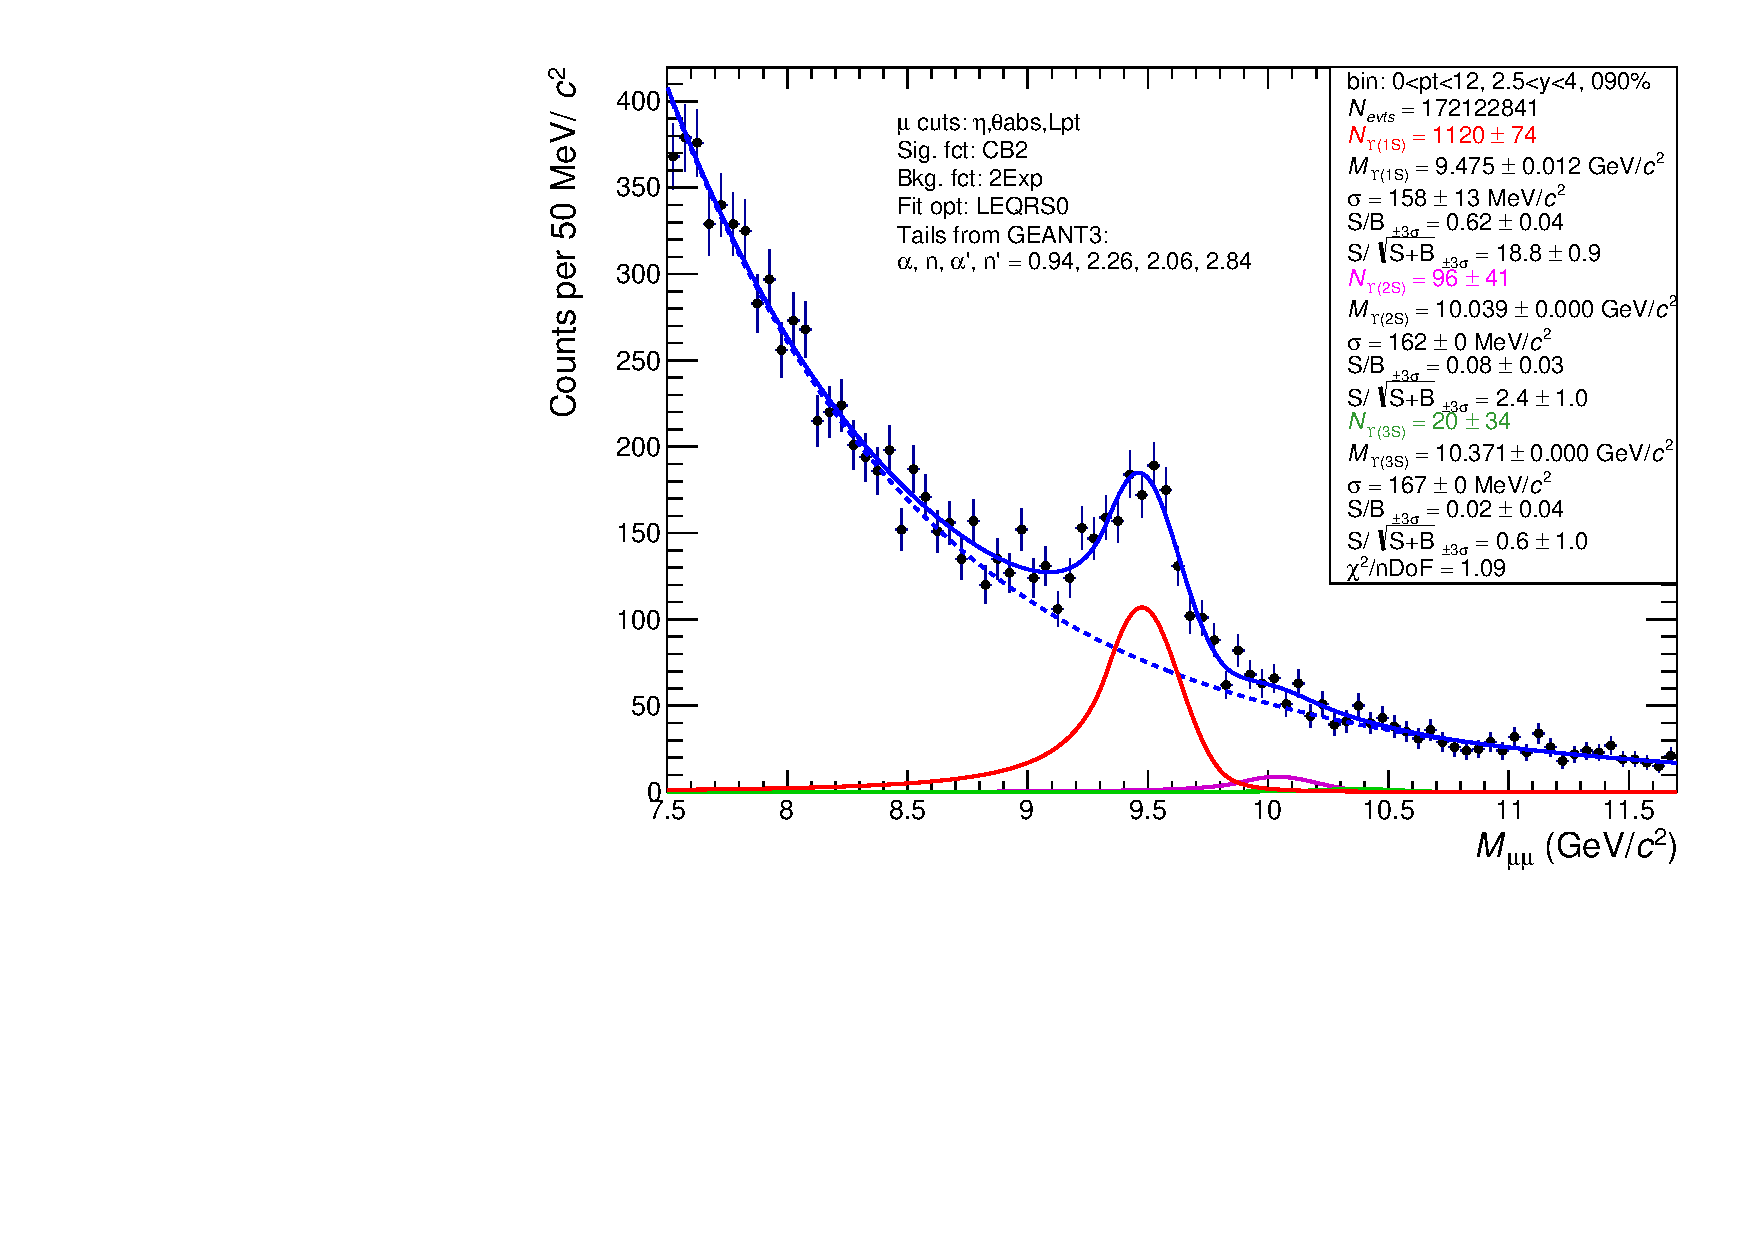
\includegraphics[width=5cm]{/Antoine/Cent/IntegralRaw.pdf}
  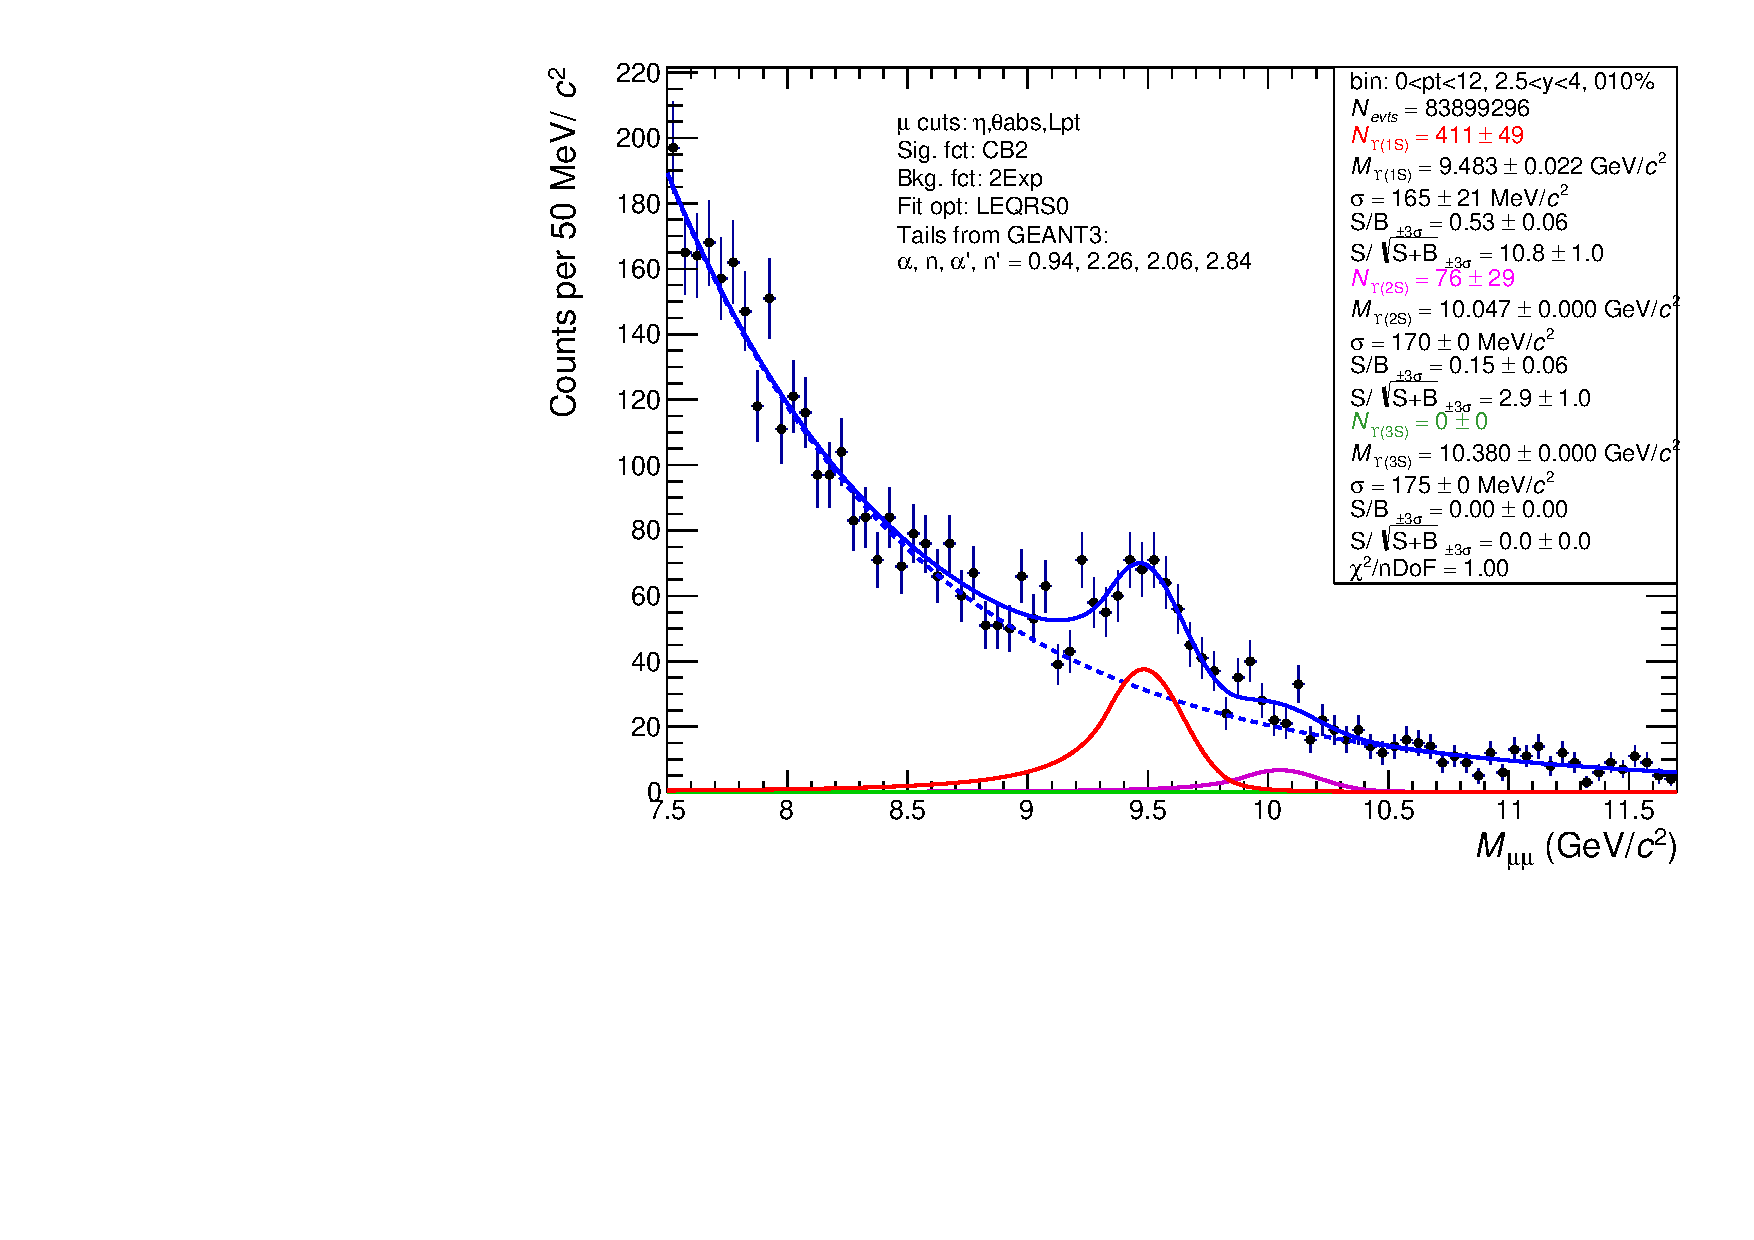
\includegraphics[width=5cm]{/Antoine/Cent/010.pdf}
  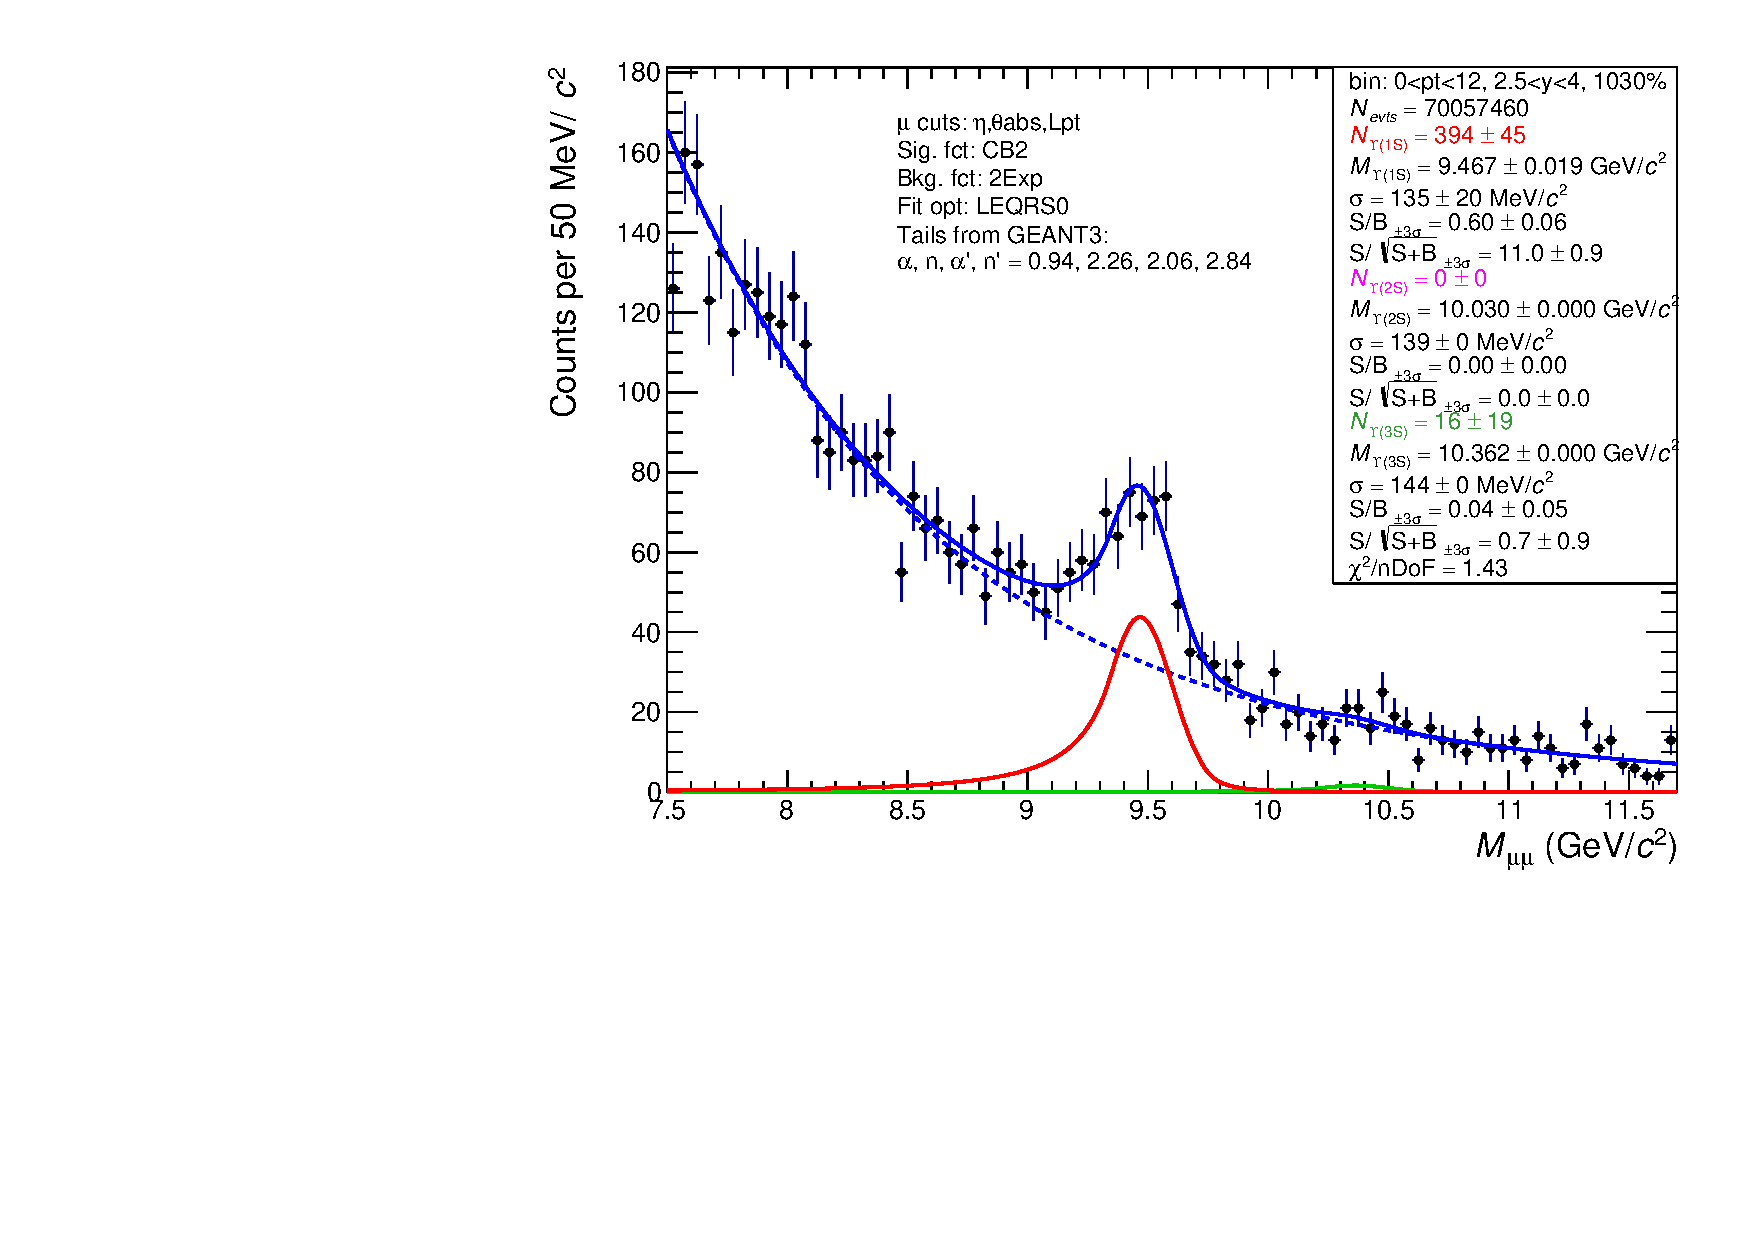
\includegraphics[width=5cm]{/Antoine/Cent/1030.pdf}
\end{figure}       

\begin{figure}[!h]
  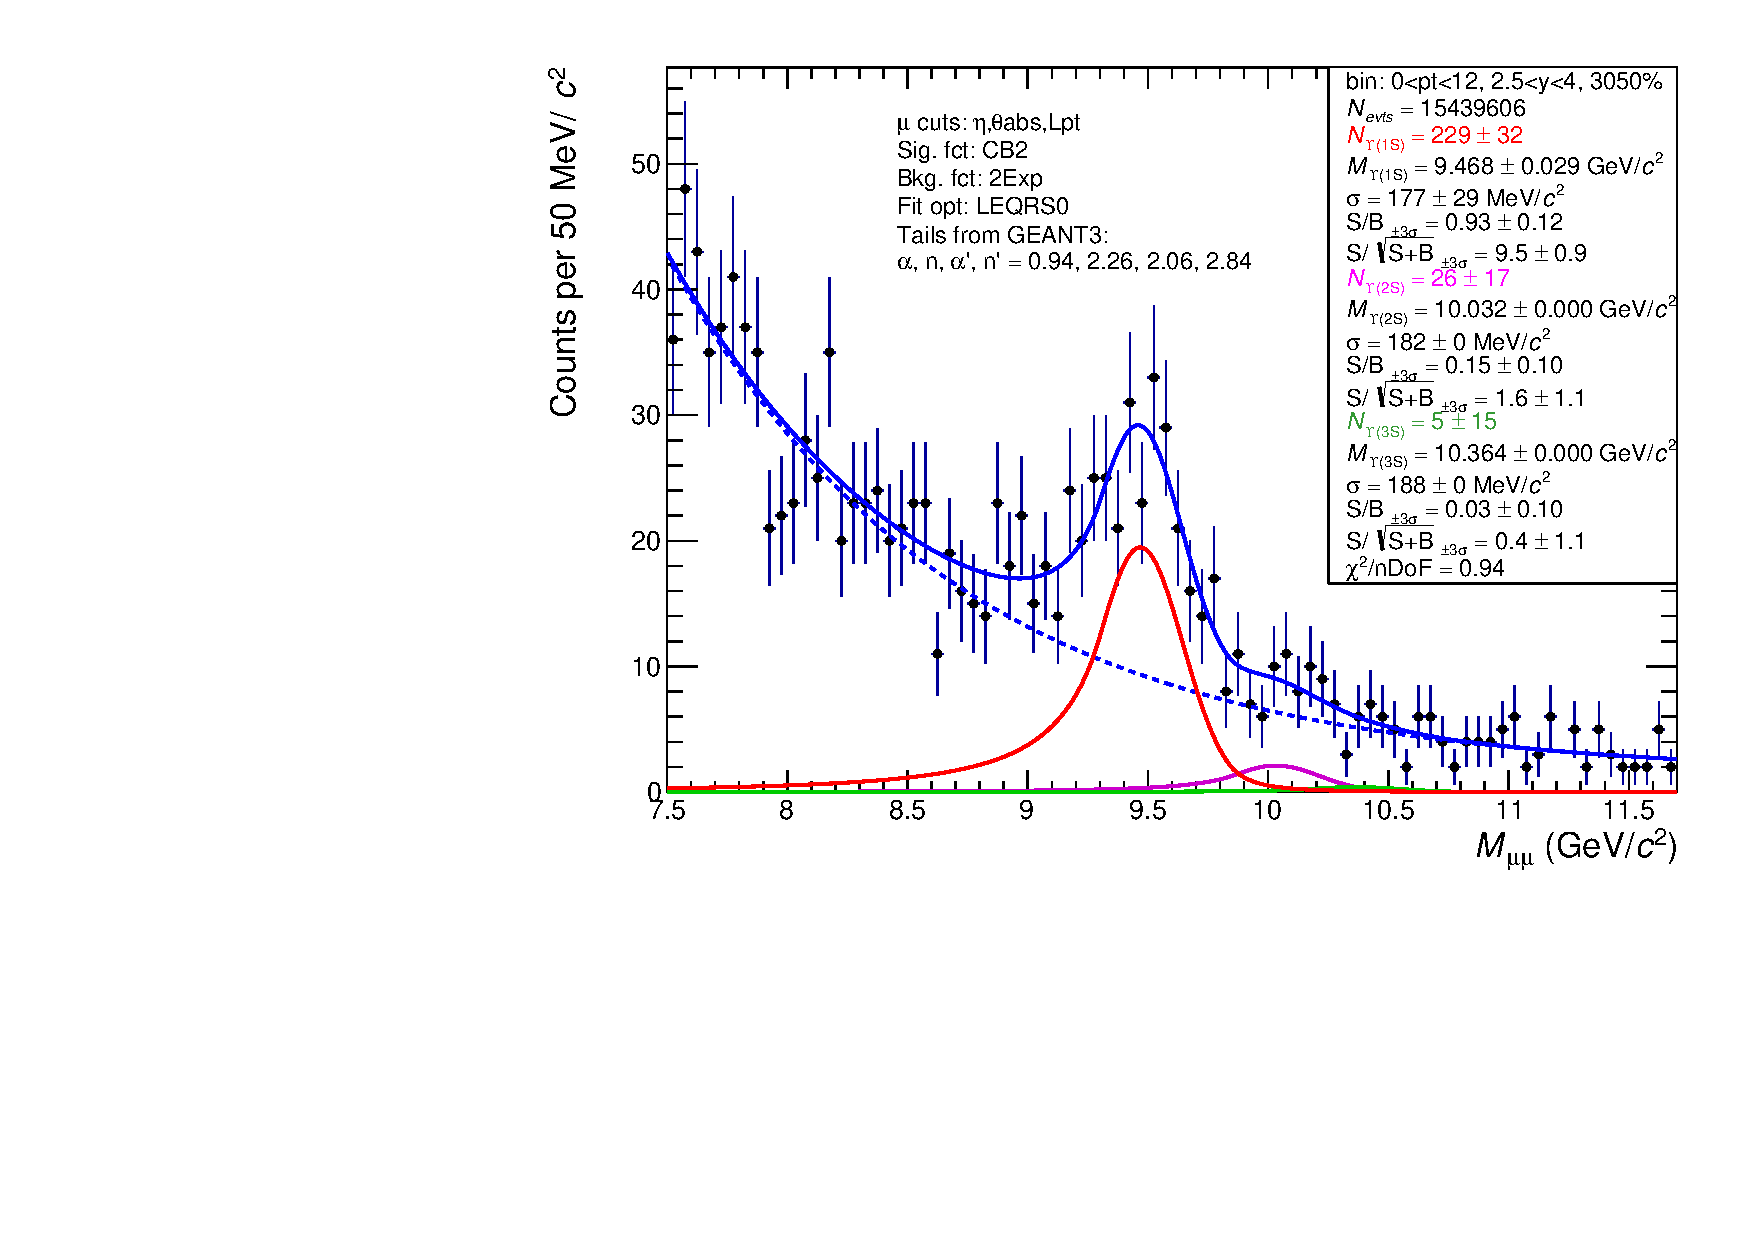
\includegraphics[width=5cm]{/Antoine/Cent/3050.pdf}
  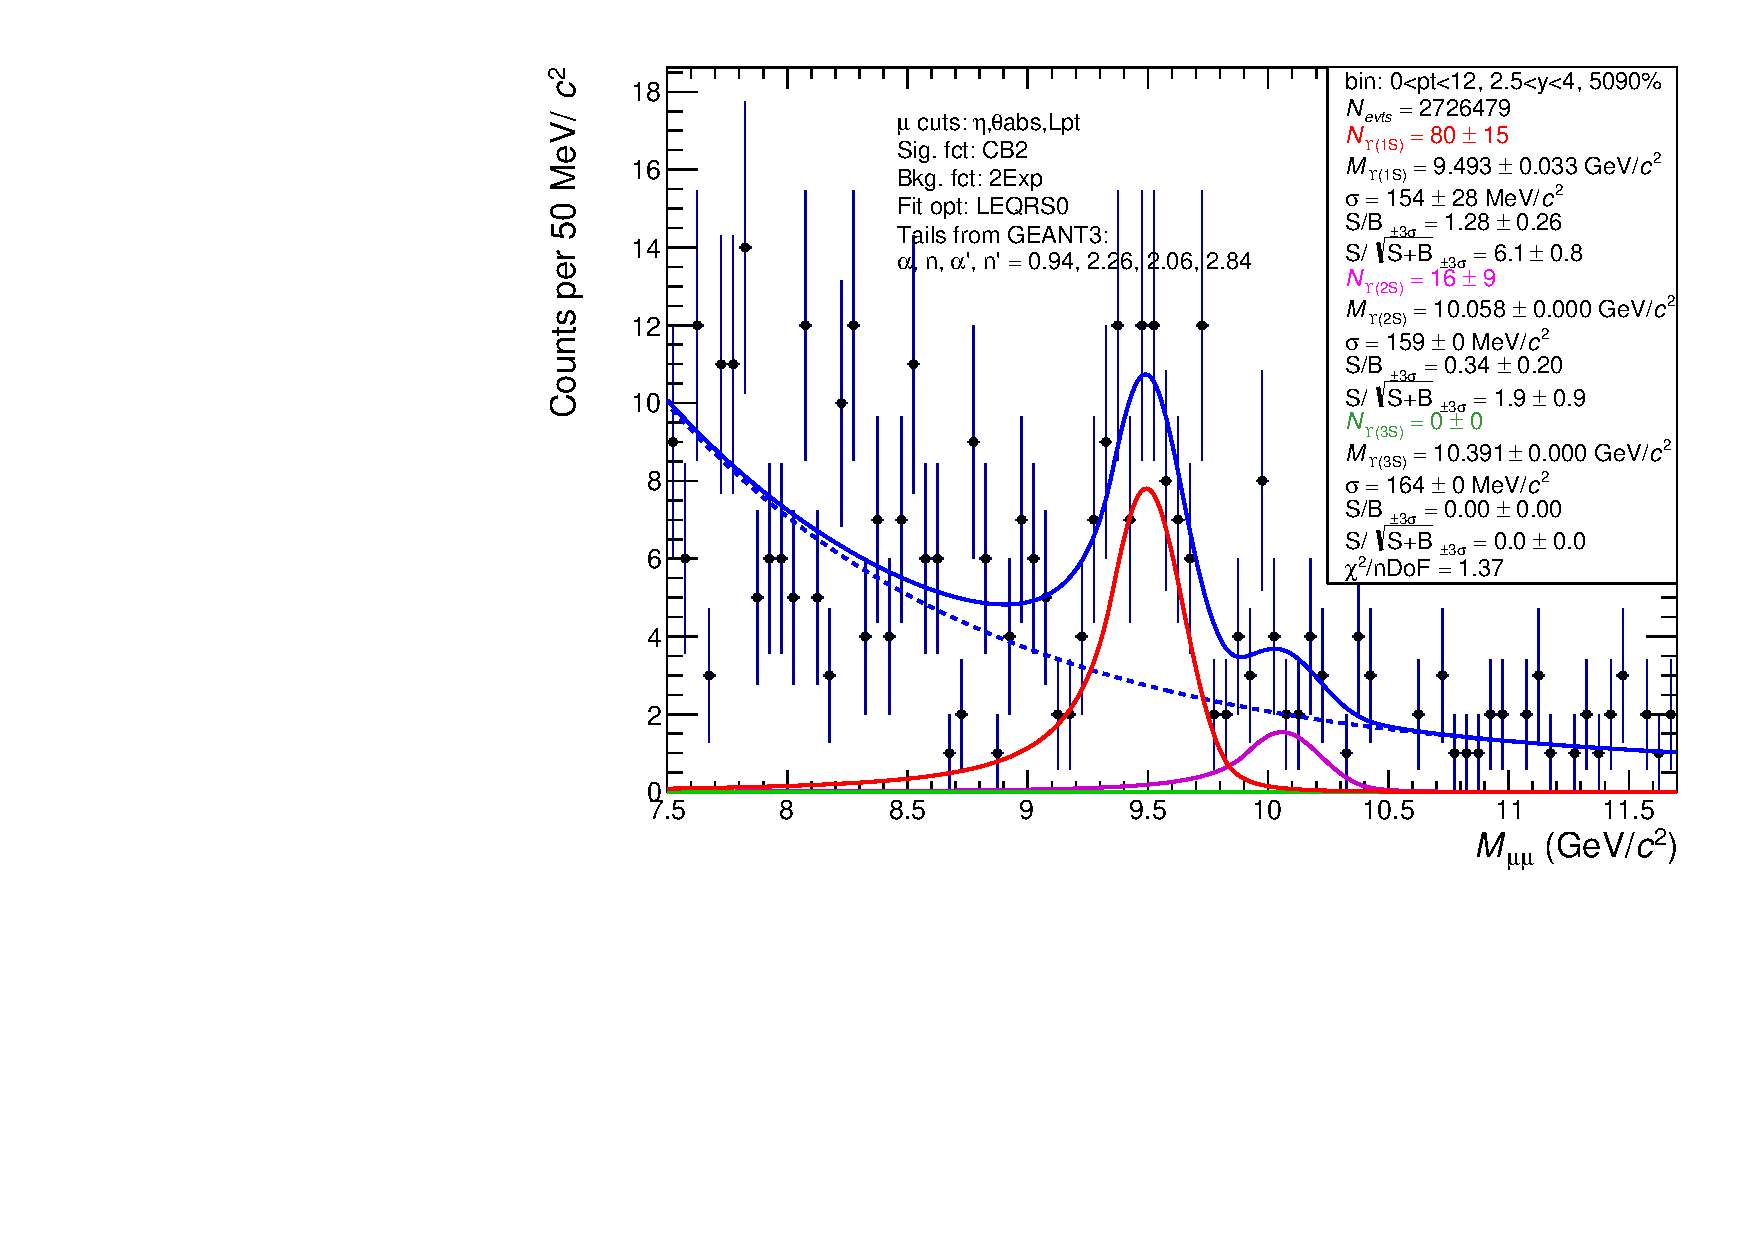
\includegraphics[width=5cm]{/Antoine/Cent/5090.pdf}
    \caption{ \label{AntoineSigCent}Signal extraction in centrality classes}
\end{figure}       

\begin{figure}[!h]
  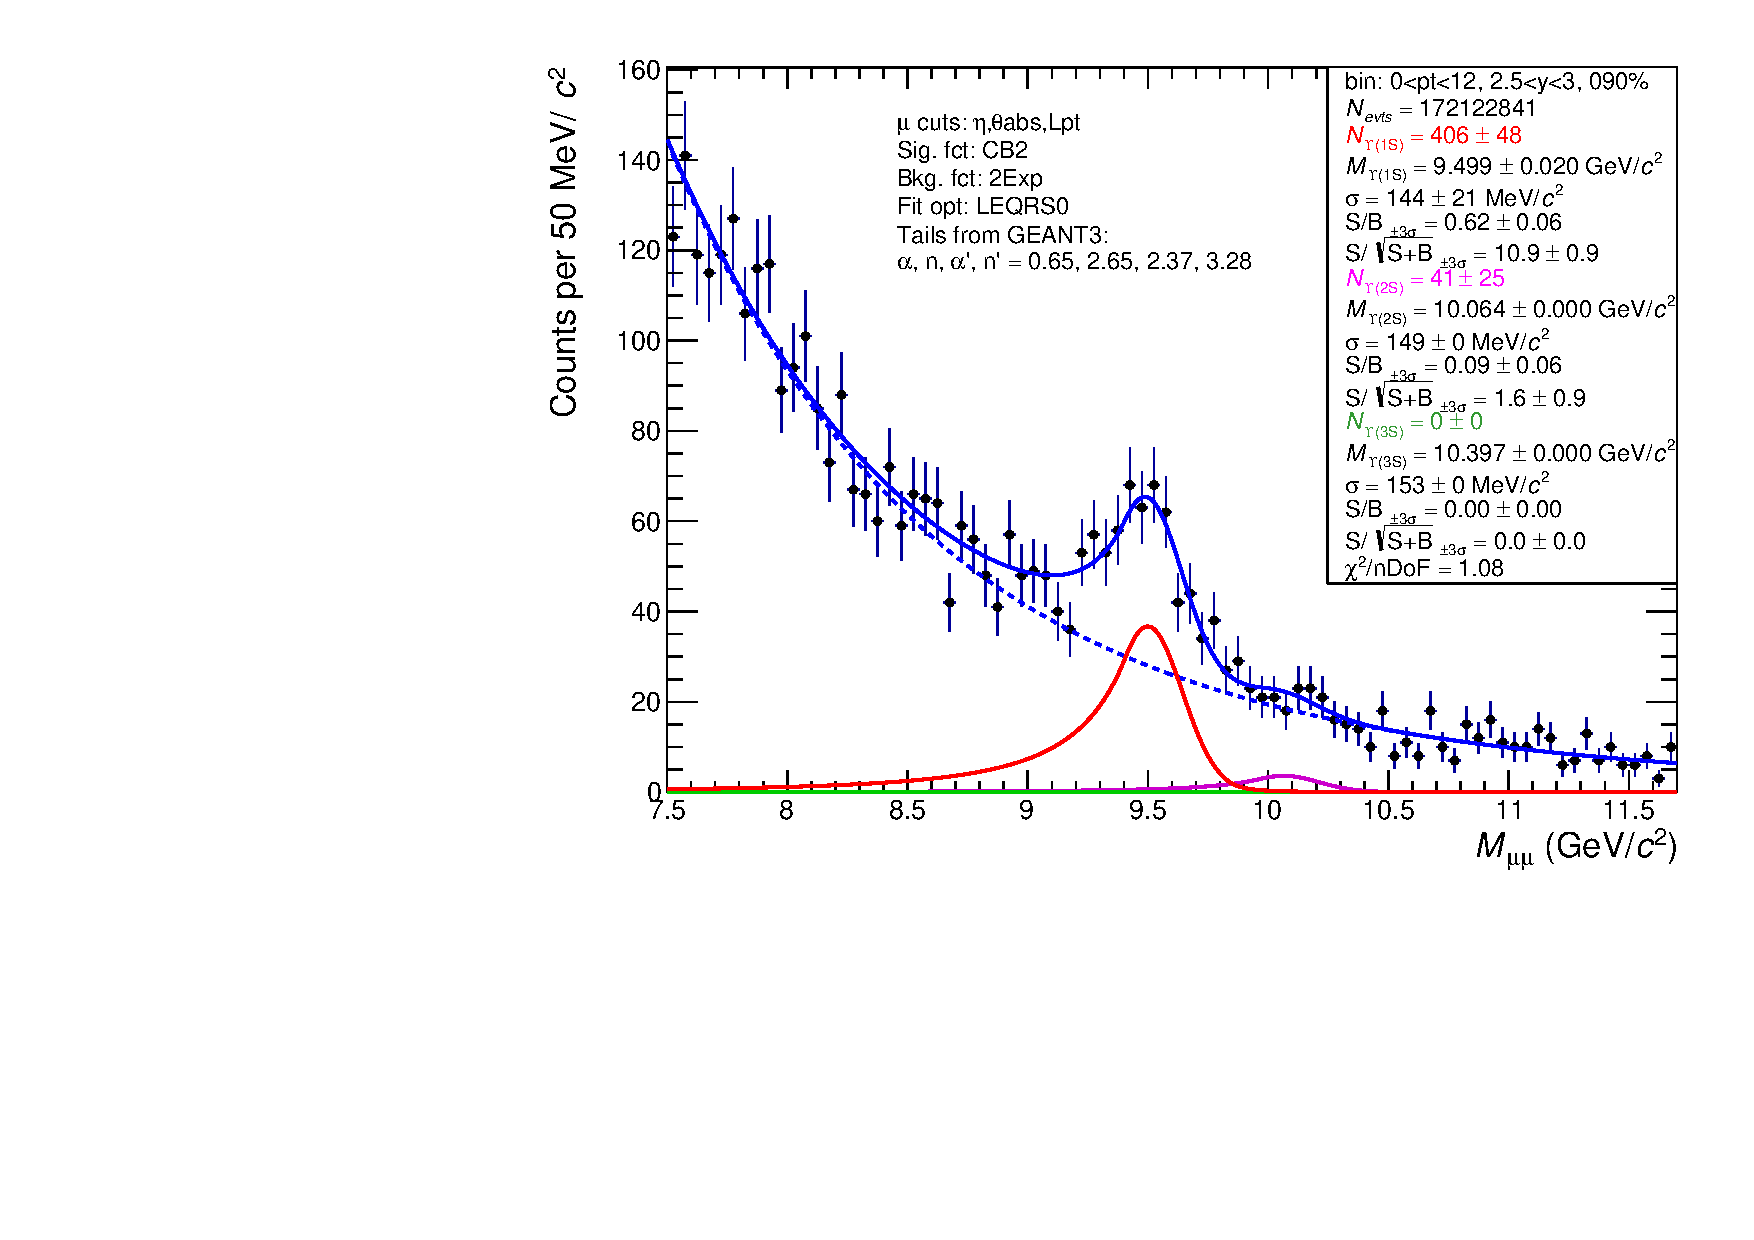
\includegraphics[width=5cm]{/Antoine/rapidity/y1.pdf}
  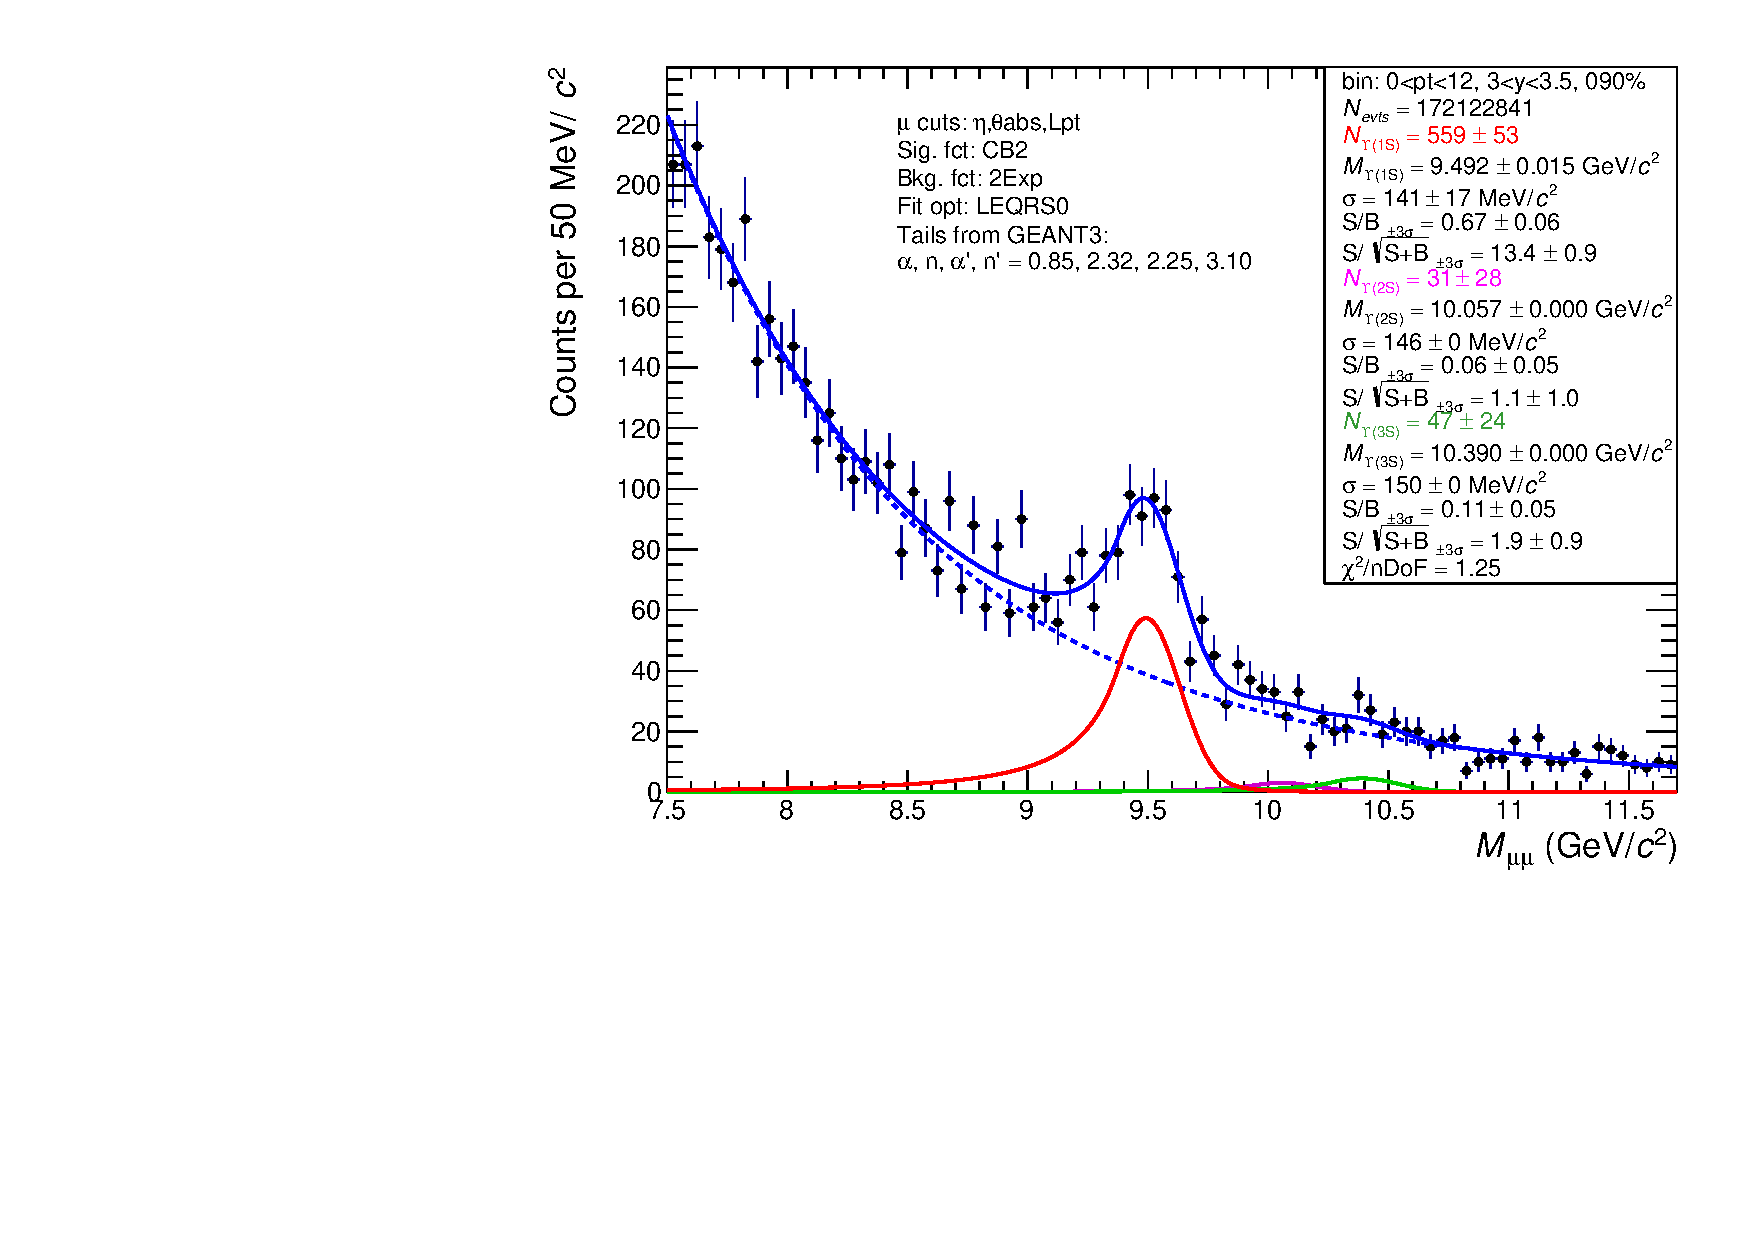
\includegraphics[width=5cm]{/Antoine/rapidity/y2.pdf}
  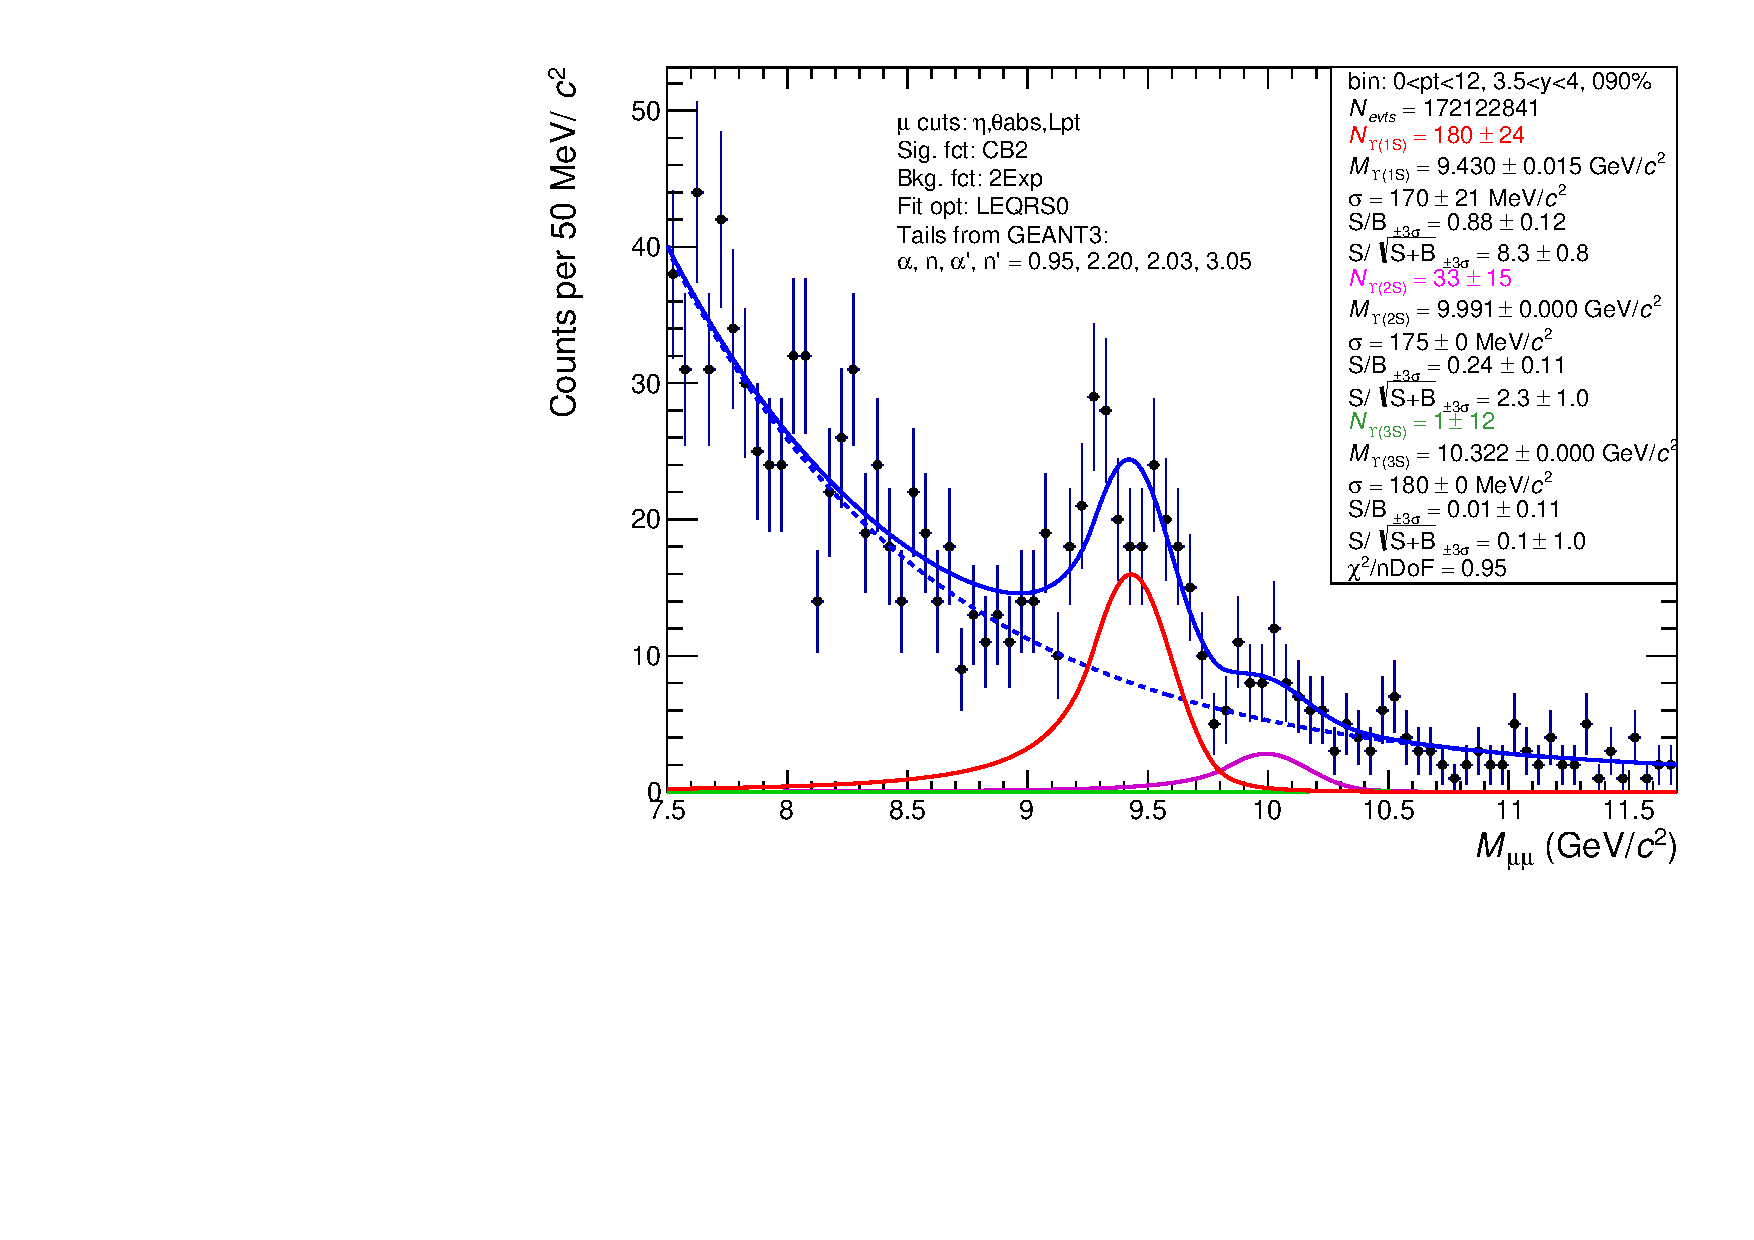
\includegraphics[width=5cm]{/Antoine/rapidity/y3.pdf}
      \caption{\label{AntoineSigY}Signal extraction in rapidity bins}
\end{figure}       



%\begin{figure}[!h]
%  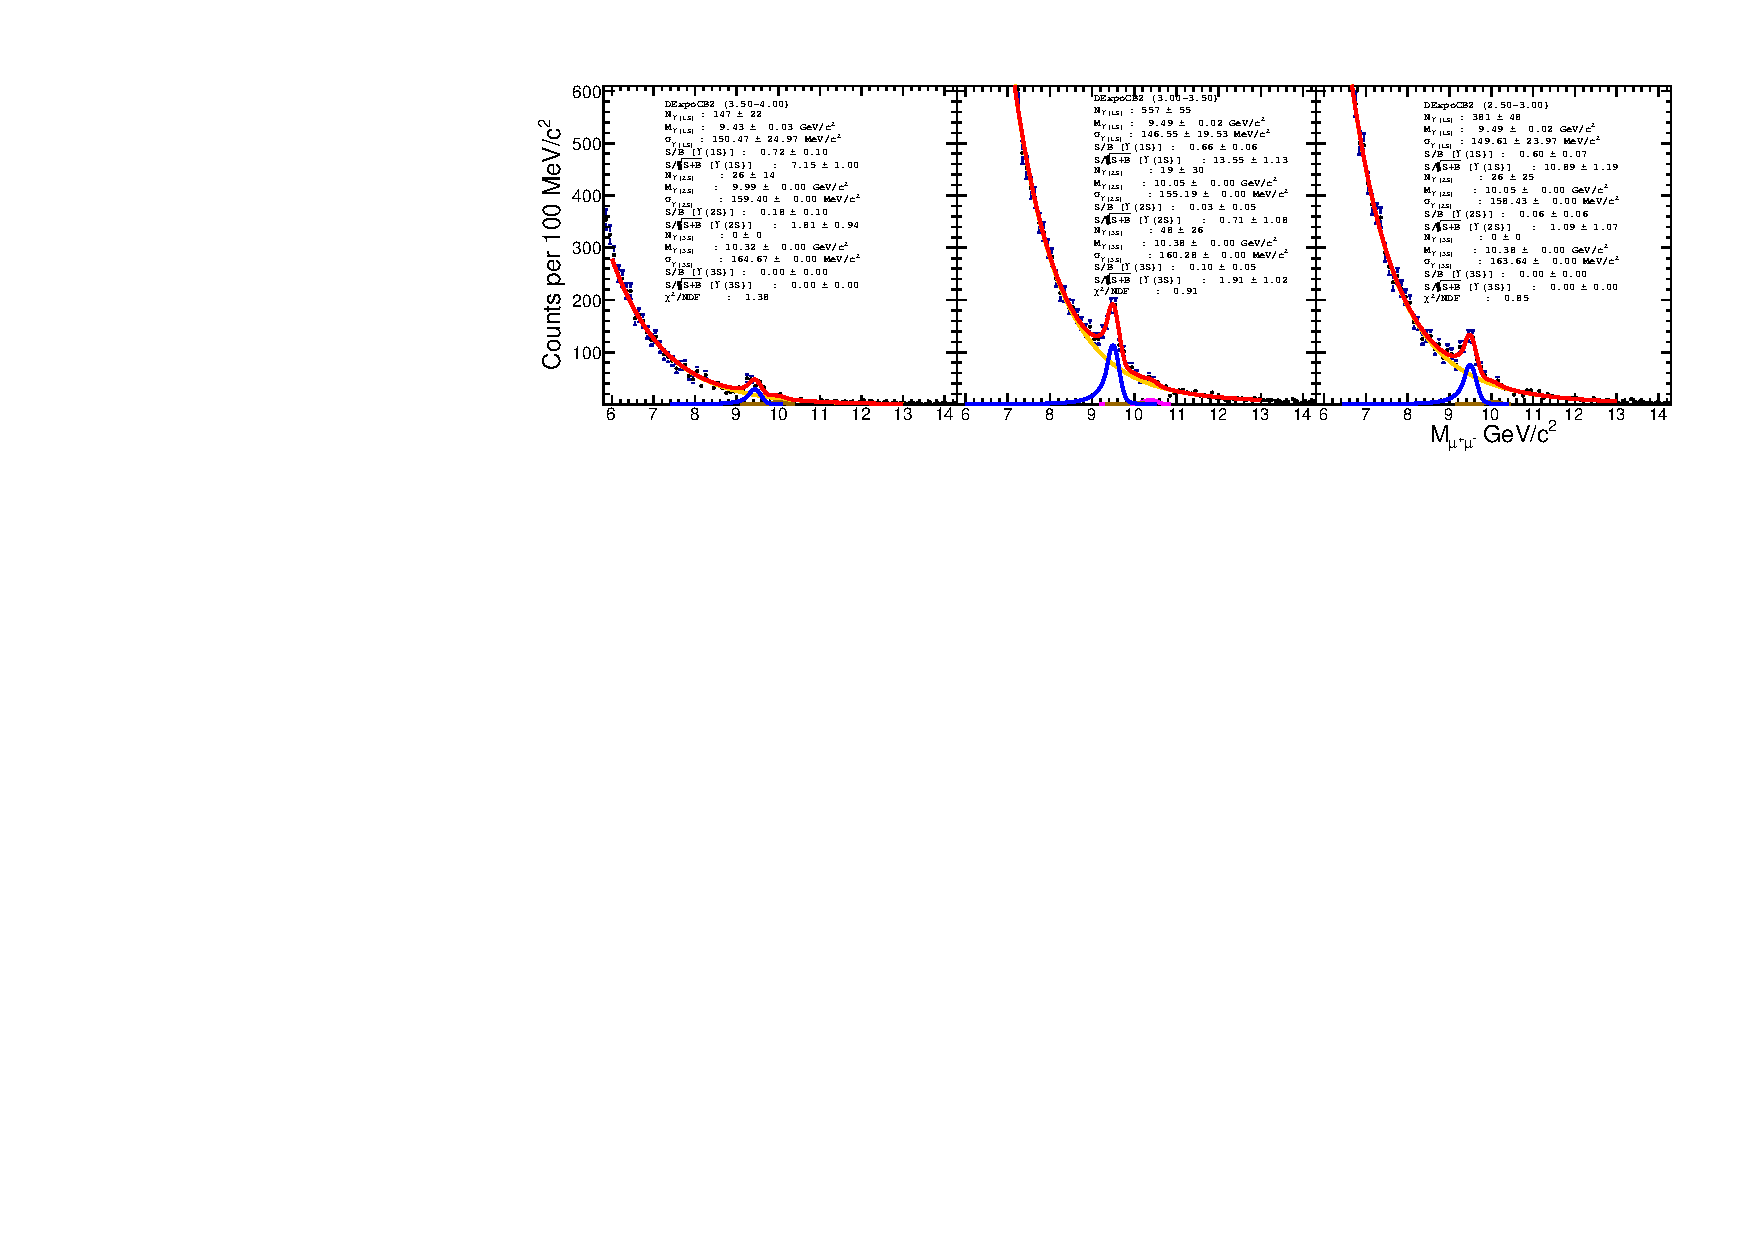
\includegraphics[width=\textwidth,height=4.0cm]{/Indra_Signal_Extraction_2016_06_08/pdca_6sig_2GeV/collection/Massfit_rap.pdf}
%\end{figure}       

%\begin{figure}[!h]
%  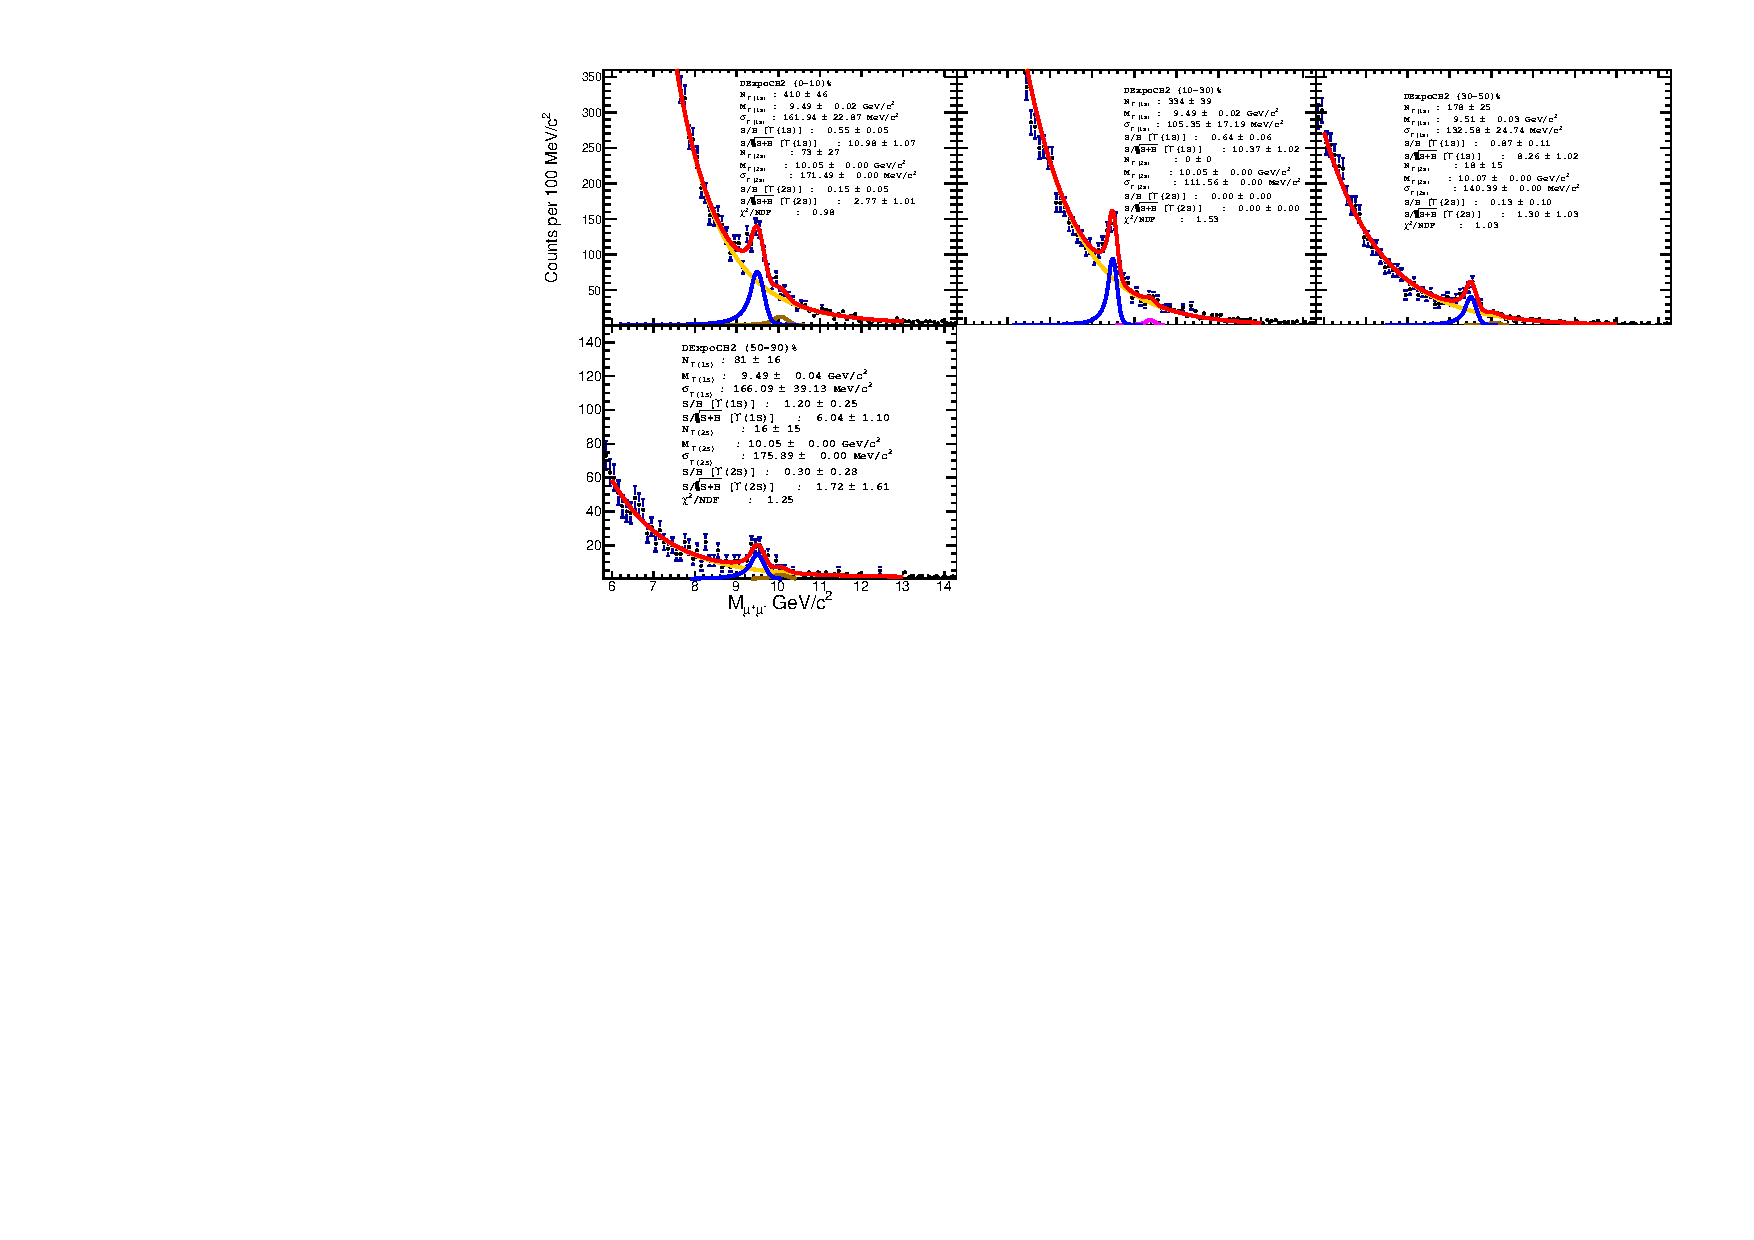
\includegraphics[width=12cm,height=7.0cm]{/Indra_Signal_Extraction_2016_06_08/pdca_6sig_2GeV/collection/Massfit_cent.pdf}
%  \caption{\scriptsize Signal in centrality bins for PDG scaling and fit range of 6-13 GeV/c}
% \end{figure}       


